% THIS IS SIGPROC-SP.TEX - VERSION 3.1
% WORKS WITH V3.2SP OF ACM_PROC_ARTICLE-SP.CLS
% APRIL 2009
%
% It is an example file showing how to use the 'acm_proc_article-sp.cls' V3.2SP
% LaTeX2e document class file for Conference Proceedings submissions.
% ----------------------------------------------------------------------------------------------------------------
% This .tex file (and associated .cls V3.2SP) *DOES NOT* produce:
%       1) The Permission Statement
%       2) The Conference (location) Info information
%       3) The Copyright Line with ACM data
%       4) Page numbering
% ---------------------------------------------------------------------------------------------------------------
% It is an example which *does* use the .bib file (from which the .bbl file
% is produced).
% REMEMBER HOWEVER: After having produced the .bbl file,
% and prior to final submission,
% you need to 'insert'  your .bbl file into your source .tex file so as to provide
% ONE 'self-contained' source file.
%
% Questions regarding SIGS should be sent to
% Adrienne Griscti ---> griscti@acm.org
%
% Questions/suggestions regarding the guidelines, .tex and .cls files, etc. to
% Gerald Murray ---> murray@hq.acm.org
%
% For tracking purposes - this is V3.1SP - APRIL 2009

\documentclass{acm_proc_article-sp}

\usepackage{times, epsfig}
\usepackage{url}
\usepackage{latexsym}
\usepackage{graphicx}
\usepackage{multirow}
\usepackage{todonotes}
\usepackage{url}
\usepackage{paralist}
\usepackage{multicol}
\usepackage{amsmath}
\usepackage{amssymb}
\usepackage{booktabs}
\usepackage{pgfplots}
\pgfplotsset{tiny,  compat=1.5}

\usepackage{amsfonts}
\usepackage{siunitx}

\begin{document}

%\title{Modeling Data Quality Rules with Markov Logic}
%\title{Effective Exploiting of Statistical Relational Learning for Data Cleaning}
\title{Using Statistical Relational Learning for Data Cleaning}

%
% You need the command \numberofauthors to handle the 'placement
% and alignment' of the authors beneath the title.
%
% For aesthetic reasons, we recommend 'three authors at a time'
% i.e. three 'name/affiliation blocks' be placed beneath the title.
%
% NOTE: You are NOT restricted in how many 'rows' of
% "name/affiliations" may appear. We just ask that you restrict
% the number of 'columns' to three.
%
% Because of the available 'opening page real-estate'
% we ask you to refrain from putting more than six authors
% (two rows with three columns) beneath the article title.
% More than six makes the first-page appear very cluttered indeed.
%
% Use the \alignauthor commands to handle the names
% and affiliations for an 'aesthetic maximum' of six authors.
% Add names, affiliations, addresses for
% the seventh etc. author(s) as the argument for the
% \additionalauthors command.
% These 'additional authors' will be output/set for you
% without further effort on your part as the last section in
% the body of your article BEFORE References or any Appendices.

\numberofauthors{5} %  in this sample file, there are a *total*
% of EIGHT authors. SIX appear on the 'first-page' (for formatting
% reasons) and the remaining two appear in the \additionalauthors section.
%
\author{
% You can go ahead and credit any number of authors here,
% e.g. one 'row of three' or two rows (consisting of one row of three
% and a second row of one, two or three).
%
% The command \alignauthor (no curly braces needed) should
% precede each author name, affiliation/snail-mail address and
% e-mail address. Additionally, tag each line of
% affiliation/address with \affaddr, and tag the
% e-mail address with \email.
%
% 1st. author
\alignauthor
Larysa Visengeriyeva\\
       \affaddr{TU Berlin}\\
       \affaddr{Germany}\\
       \email{fn.ln@tu-berlin.de}
\alignauthor
Alan Akbik\\
       \affaddr{TU Berlin}\\
       \affaddr{Germany}\\
       \email{fn.ln@tu-berlin.de}
\alignauthor
Sebastian Schelter\\
       \affaddr{TU Berlin}\\
       \affaddr{Germany}\\
       \email{fn.ln@tu-berlin.de}
\and%
\alignauthor
Manohar Kaul\\
       \affaddr{TU Berlin}\\
       \affaddr{Germany}\\
       \email{fn.ln@tu-berlin.de}
\alignauthor
Volker Markl\\
       \affaddr{TU Berlin}\\
       \affaddr{Germany}\\
       \email{fn.ln@tu-berlin.de}
}


\maketitle
\begin{abstract}
High quality data is important for data science methods. Unfortunately,  digitally collected data often suffers from many data quality issues, such as duplicate, incorrect or incomplete data. A common approach for counteracting such issues is to formulate a set of data agnostic cleaning rules intended to identify and repair incorrect, duplicate and missing data. There is also a need for new approaches to overcome the limits of existing heuristic data cleaning solution. In this paper, we address this issue by proposing an approach to data cleaning based on Statistical Relational Learning (SRL) and probabilistic inference. We argue that a well-known formalism - Markov logic - is a natural fit for modeling interacting data quality rules in a flexible and extensible way. We show how data quality rules expressed as first-order formulas can be directly translated into a predictive model in an SRL framework. This approach allows the usage of probabilistic joint inference over interleaved data cleaning rules to improve data quality. In an experimental study we demonstrate the viability of our proposed approach.
\end{abstract}


%%%%%%%%%%%%%%%%%%%%%%%%%%%%%%%%%%%%%%%%%%%%%%%%%%%%%%%%%%%%%%%%%%%%%%%%
% Introduction
%%%%%%%%%%%%%%%%%%%%%%%%%%%%%%%%%%%%%%%%%%%%%%%%%%%%%%%%%%%%%%%%%%%%%%%%
\section{Introduction}
\label{sec:intro}

\todo[inline]{in order to contribute to data quality improvement, data cleaning should be done on real world data (see the The Data Tamer System paper)}
\todo[inline]{add a clear statement what is new}

%What is the problem?
% see here for description why data quality is important.
% http://books.google.de/books?hl=en&lr=&id=SULMBFgtwQoC&oi=fnd&pg=PA1&ots=uaNGyVfL7V&sig=RER31QotCCRJeaQq8OafAtpgK1k#v=onepage&q&f=false
Having access to high quality data is of great importance in data analysis. However, data in the real world is often considered \textit{dirty}: it contains inaccurate, incomplete, inconsistent, duplicated, or stale values~\cite{chu2004blissful}. A number of distinct data quality issues are known in the field of data quality management such as \textit{data consistency}, \textit{currency}, \textit{accuracy}, \textit{deduplication} and \textit{information completeness}~\cite{fan2012foundations}. As previous work has observed, such data quality issues are detrimental to data analysis~\cite{national2013Frontiers,Fan:2008:CFD:1366102.1366103} and cause huge costs to busi\-nesses \cite{waynew.eckerson2002}. Therefore, improving data quality with respect to business and integrity constraints is a crucial component of data management. 
A common approach to increase data quality is to formulate a set of \textit{data cleaning rules} that detect semantic errors by utilizing data dependencies~\cite{fan2012foundations, Arasu:2009:LDC:1546683.1547340, Dallachiesa:2013:NCD:2463676.2465327, llunaticVDLB2013b}. However, previous research identified a number of requirements and accompanying challenges, which are associated with creating such rule sets (c.f., Section~\ref{sec:frontiers}): 

%\todo[inline]{Desiderata: Challenge}  
\textit{Interleaved rules}. First, while each such rule usually addresses one data quality issue individually, the individual rules as a whole typically \textit{interact}~\cite{fan2012foundations, Fan:2014:IRM:2628135.2567657}. For instance, a rule that deletes duplicates might perform better after missing data has already been imputed, while, on the other hand, a rule that imputes missing data might perform better if duplicates have already been removed. Therefore, we argue to model data quality rules such as deduplication and missing value imputation \textit{jointly}, rather than as separate processes.
Second, rules in such a rule-set may need to be modeled \textit{"soft"} and \textit{"hard"} in order to balance constraints of different importance \cite{Yakout:2013:DSU:2463676.2463706}, especially within a set of interacting rules. 

\textit{Automation}. Different execution orders of interleaved rules produce different results~\cite{Dallachiesa:2013:NCD:2463676.2465327}. Imposing the difficult problem of manually specifying the execution order on the user conflicts with the automation principle of data curation systems~\cite{Stonebraker_datacuration}.

\textit{Usability and domain knowledge integration}. Various languages and statistical approaches for data curation exist \cite{Dallachiesa:2013:NCD:2463676.2465327, chu2013holistic, llunaticVDLB2013b}. However, there is a need for expressiveness and customization of the rules in order to integrate arbitrary constraints into data cleaning without having to specify complex user-defined functions. 

In this paper, we present an approach to data cleaning based on statistical relational learning (SRL)~\cite{getoor2007introduction} and probabilistic inference~(c.f.,~Section~\ref{sec:method}). SRL is a branch of machine learning that models joint distributions over relational data. Generally, data quality rules represent relationships between attributes in the database schema (c.f., Section~\ref{sec:expl}). These rules are mainly based on integrity constraints such as functional dependencies~\cite{AbiteboulHV95, fan2012foundations} on top of a database schema. We show how to translate such functional dependencies, expressed as first-order logic formulas, into probabilistic-logical languages, which allows us to reason over inconsistencies, duplicates or missing values in a probabilistic way~(c.f.,~Section~\ref{sec:ml}). During automatic data cleaning, the optimal order of rules execution is hardly achievable \cite{Dallachiesa:2013:NCD:2463676.2465327}. Therefore, we propose to use joint inference for the simultaneous rules execution.

The contributions of this paper are the following:

\begin{itemize}
  \item We discuss how to model data cleaning rules based on integrity constraints within the probabilistic framework of\\ Markov~logic~(Section~\ref{sec:ml}).
  \item We describe how data repair leverages joint inference on probabilistic graphical models and allows us to treat data curation rules holistically, which obliterates the need to specify execution order (Section~\ref{subsec:jointinference}).\\
 \item We present an extensive empirical study of holistic modeling and error prediction in data cleaning using Markov logic. Modelling data quality rules in a probabilistic way enables statistical inference of data quality errors. Our experimental evaluation reveals that the simultaneous treatment of data cleaning rules leads to higher accuracy in data curation. We show that joint inference for data correction prediction outperforms sequential execution of data cleaning rules on a dataset comprised of hundred thousands tuples with $10\%$ of noisy values, and results in an improved $F_1$-score of $0.95$ (Section~\ref{sec:evaluation}).
\end{itemize}


%%%%%%%%%%%%%%%%%%%%%%%%%%%%%%%%%%%%%%%%%%%%%%%%%%%%%%%%%%%%%%%%%%%%%%%%
% Data Cleaning Rules
%%%%%%%%%%%%%%%%%%%%%%%%%%%%%%%%%%%%%%%%%%%%%%%%%%%%%%%%%%%%%%%%%%%%%%%%
\section{Data Quality Fundamentals}
\label{sec:expl}
In this section, we explain the notation and underlying theory to the data cleaning problem. We consider a database instance $\mathcal{D}$ with a relational schema $\mathcal{S}$. $\mathcal{D}$ contains a relation $\mathcal{R} \in \mathcal{S}$ that is defined for the set of attributes $attr(\mathcal{R})$. $dom(U_i)$ denotes the domain of an $i$-th attribute with $U_i \in attr(\mathcal{R})$. For data cleaning, we leverage a set of data quality rules, which are data-agnostic and rely on data integrity constraints~\cite{AbiteboulHV95, fan2012foundations}.

A \textbf{functional dependency} (FD) on a relational schema $S$ is an expression of the form $\phi: X \rightarrow Y$ where $X \subseteq attr(\mathcal{R}) $ and $Y \subseteq attr(\mathcal{R})$. % are subsets of $\mathcal{R}'s$ attributes $attr(\mathcal{R})$. 
An FD holds if every pair of tuples of $\mathcal{R}$ that match on each of the attributes in $X$, also match on the attributes in $Y$. Data quality management systems leverage functional dependencies to find and correct dirty data, because these dependencies specify the semantics of the data in a declarative way. The main disadvantage of functional dependencies is that they operate solely on the schema level and are often not able to detect conflicts in real-life data. This is because FDs do not capture a subset of data but instead always operate globally on the whole dataset.
Therefore, we consider an extension of traditional functional dependencies:  A \textbf{conditional functional dependency} (CFD) 
defined on the relational schema $\mathcal{S}$ is a pair $\psi(X \rightarrow Y , T_p)$,  where $X \rightarrow Y$ is a standard 
FD and $X \cup Y \subseteq attr(\mathcal{R})$ and $T_p$ is a tuple pattern, which is a set of constraints holding on the particular 
subset $X \cup Y$ of tuples. For each $U \in X \cup Y$, the value of the attribute $U$ for $T_p$, $T_p[U]$ is either a variable 
value $`\_`$, or a constant $u \in dom(U)$. Data deduplication techniques use FDs to define matching dependencies. The 
difference is that matching dependencies use the notion of a similarity predicate instead of an equality predicate. A 
\textbf{Matching Dependency} (MD) for schemas $\mathcal{S}_1$ and $\mathcal{S}_2$ is syntacticly defined as:
$\mu: \mathcal{S}_1[X_1]\approx \mathcal{S}_2[X_2]\rightarrow \mathcal{S}_1[Y_1]\rightleftharpoons \mathcal{S}_2[Y_2]$ 
where $X_1 \cup Y_1$ and $X_2 \cup Y_2$ are pairwise compatible sets of attributes in $attr(\mathcal{R}_1), \mathcal{R}_1\in \mathcal{S}_1$ 
and $attr(\mathcal{R}_2), \mathcal{R}_2\in \mathcal{S}_2$, respectively; $\approx$ indicates similar attributes and $\rightleftharpoons$ 
is called the \textit{matching operator}. In other words the matching operator $\rightleftharpoons$ indicates that $t_1[Y_1]$ and $t_2[Y_2]$ refer to the same real-world entity for each tuple $t_1$ from $\mathcal{S}_1$  and each tuple $t_2$ from $\mathcal{S}_2$. A MD has dynamic semantics, meaning it points out \textit{how} to repair data. Hence, MDs force to update $t_1[Y_1]$ and $t_2[Y_2]$ such that they have the same values. % \note{unclear and incorrect english, rewrite sentence}. -done
The operator $\rightleftharpoons$ only requires that the $t_1[Y_1]$ and $t_2[Y_2]$ are identified.

\section{Frontiers in Data Cleaning}
\label{sec:frontiers}

Next, we showcase limitations of rule-based data cleaning. Therefore, we introduce the following data cleaning scenario:
\label{sec:example}
% CUSTOMER
\begin{table}[h]\footnotesize
\scriptsize
\resizebox{\columnwidth}{!}{%
\begin{tabular}{lllllll} \toprule 
\textbf{id} &  \textbf{firstname} & \textbf{lastname} & \textbf{street} & \textbf{city} & \textbf{zipcode} & \textbf{phone} \\ \midrule
$c_1$ & Ron & Howard & 1 Sun Dr. & Los Angeles & 90001 & 12345 \\
$c_2$ & Max & Miller & 12 Hay St. & Napa & 94558 & 11234 \\ \bottomrule
\end{tabular}}
\vspace{-1em}
\caption{\textsc{customer} table (with errors)}
\label{tab:cust}
\end{table}

% TRANSACTION
\begin{table}[h]\footnotesize
\scriptsize
\resizebox{\columnwidth}{!}{%
\begin{tabular}{llllllll} \toprule 
\textbf{id} & \textbf{item} &  \textbf{firstname} & \textbf{lastname} & \textbf{street} & \textbf{city} & \textbf{zipcode} & \textbf{phone} \\ \midrule
$t_1$ & iPhone6 & R. & Howard & 1 Sun Dr. & L.A. & null & null \\
$t_2$ & Galaxy5 & null & Miller & 12 Hay St. & null & 94558 & 11234 \\
$t_3$ & Nexus5 & Howard & Ron & null & null & 90001 & 12345 \\ \bottomrule
\end{tabular}}
\vspace{-1em}
\caption{\textsc{transaction} table (with errors)}
\label{tab:trans}
\end{table}


Consider the following relational tables: the \textsc{customer} table (c.f.,~Table~\ref{tab:cust}) 
records address and contact details of each customer. The \textsc{transaction} table (c.f.,~Table~\ref{tab:trans}) 
records each purchased item, together with the personal details entered by the customer during the purchase. 
The example data has several quality issues: (1) Missing values in the \textsc{transaction} table, indicated by \emph{null} values; (2) false values, e.g.,  the customer ``Ron Howard'' is involved in transaction $t_3$ , but in the transaction table his name is falsely recorded as ``Howard Ron''; (3) duplication issues, e.g., the city of ``Los Angeles'' is sometimes entered into the table as ``L.A.'' and the first name ``Ron'' is once abbreviated as ``R.''. 

%Note: I would not call (3) as duplication, since it is across different tables. 

In order to correct these issues, we need to identify the corresponding entries for each transaction in the \textsc{customer} table and use these to automatically clean the transaction data. Although enough information exists to make such links possible through manual linking, defining automatic cleaning rules to accomplish this task is not trivial. For instance, a hard rule that states that $\textsl{city}$ field values ``L.A.'' and ``Los Angeles'' are always the same, intuitively makes sense. Yet, this assumption does not hold for the $\textsl{firstname}$ values ``R.'' and ``Ron''. Rather, we would need a \emph{soft rule} that indicates that both strings \emph{possibly} refer to the same entity, but that we may require additional evidence. Next, consider the \emph{null} value in $t_1.$\textsl{zipcode}. We would like to fill this missing value by linking the transaction to customer $c_1$, but only the fields \textsl{lastname} and \textsl{street} fully match, while \textsl{city} (and possibly \textsl{firstname}) may match using the de-duplication rules mentioned above. Even though this provides significant evidence that the transaction should be linked to customer $c_1$, there is still a chance that two different people share the same last name and street address in a large city. Inclusion of the \textsl{phone} field into the rule would make us reasonably certain that they should be linked, but as the example shows, the value for this field is missing. 

This example illustrates the limitations of data cleaning via hard rules: Because the example table is heavily corrupted, it is very hard to define data cleaning rules, which do not introduce errors. Instead, we would prefer to define a number of \emph{soft rules} that aggregate evidence. Examples include first name abbreviation rule (``R.'' vs. ``Ron''), a first and last name switch rule (indicating that there is a small chance that ``Ron Howard'' and ``Howard Ron'' are the same person), and rules that indicate that the more fields two tuples in the \textsc{customer} and \textsc{transaction} tables share, the more likely it is that they refer to the same person. 

The functional dependency: $\textsl{fd}: \textsc{transaction}([\textsl{city}, \textsl{phone}] \rightarrow [\textsl{street}, \textsl{zipcode}])$ declares that, in the \textsc{transaction} table, the two fields \textsl{city} and \textsl{phone} together 
uniquely determine the two fields \textsl{street} and \textsl{zipcode}. Although two instances of the customer ``Ron Howard'' in ~Table~\ref{tab:trans} are recorded, one is missing the \textsl{phone} value. In this case, the rule only applies when combined with additional data cleaning rules. The rule $\textsl{cfd}: \textsc{transaction}([\textsl{zipcode}] \rightarrow [\textsl{city}], T_1 =(90001~||~\text{Los~Angeles}))$ states that every tuple in which the value for \textsl{zipcode} equals $90001$ must have its \textsl{city} attribute set to ``Los~Angeles". In our example in Table~\ref{tab:trans}, this rule corrects the \emph{null} value in transaction $t_3$. 

For the \textsl{firstname} field in transaction $t_1$ in Table~\ref{tab:trans}, we could define a rule indicating that the values ``R.'' and ``Ron'' refer to the same name, but cannot always be certain whether this is the case. To include additional evidence, we create the following MD to link transaction $t_1$ to customer $c_1$:\\ 
%$ \textsl{md}: \textsc{transaction}[\textsl{lastname}, \textsl{city}, \textsl{street}] = \textsc{customer}[\textsl{lastname}, \textsl{city}, \textsl{street}] \land \textsc{t}[\textsl{firstname}] \approx \textsc{customer}[\textsl{firstname}]  \rightarrow \textsc{transaction}[\textsl{firstname}] \rightleftharpoons \textsc{customer}[\textsl{firstname}]$
\vspace*{-0.5cm}
\begin{table}[h]\footnotesize
\scriptsize
\centering
\resizebox{\columnwidth}{!}{%
%\begin{tabular}{l}
\begin{tabular}[c]{@{}c@{}}
$ \textsl{md}: \textsc{transaction}[\textsl{lastname}, \textsl{city}, \textsl{street}]
= \textsc{customer}[\textsl{lastname}, \textsl{city}, \textsl{street}] $ \\
$\land \textsc{transaction}[\textsl{firstname}] \approx \textsc{customer}[\textsl{firstname}] $ \\
$ \rightarrow \textsc{transaction}[\textsl{firstname}] \rightleftharpoons \textsc{customer}[\textsl{firstname}]$

%\end{tabular}
\end{tabular}}
\end{table}
\vspace*{-0.5cm}

This MD states that if any two tuples from \textsc{transaction} and \textsc{customer} match on \textsl{lastname}, \textsl{city}, \textsl{street}, and their \textsl{firstname} values are similar, then \textsc{transaction}[\textsl{firstname}] and \textsc{customer} [\textsl{firstname}] should have the same values. This rule shows how the notion of similarity may be included in rules, but only within first-order logic, i.e., the similarity condition is either \emph{true} or \emph{false}. In reality, we are able to determine a more fine graded similarity, i.e., some types of similarity that we deem to be more probable (``L.A.'' and ``Los Angeles''), and others that are less probable (``R.'' and ``Ron''). Moreover, we may have different levels of confidence regarding functional or matching dependencies that we define. The above rule for the example is very likely, but not necessarily always true. However, hard first-order logic does not permit us to formalize this intuition, as it does not allow for a probabilistic interpretation of the rules.

%%%%%%%%%%%%%%%%%%%%%%%%%%%%%%%%%%%%%%%%%%%%%%%%%%%%%%%%%%%%%%%%%%%%%%%%
% Approach
%%%%%%%%%%%%%%%%%%%%%%%%%%%%%%%%%%%%%%%%%%%%%%%%%%%%%%%%%%%%%%%%%%%%%%%%
\section{Proposed Approach}
\label{sec:method}

\note{This intro here must be much more concrete, it is too general and high level. Also, it is very long.}

% \begin{figure}[t]
% \centering
% \includegraphics[width=200px, height=140px]{img/system.pdf}
% \caption{\anno{Rmove this picture?} Our proposed method for data cleaning based on Markov logic consists of three main components: 
% (I) A \textbf{Rule-based Data Quality Management} component that is based on the data quality rules to address different data quality issues;
% (II) A \textbf{relation prediction} component based on probabilistic inference performed by the Markov logic framework and (III) 
% a \textbf{Data Layer} that includes a number of data sources including relational and semi-structured data.}
% \label{fig:system}
%\end{figure}     

Our proposed approach is to model data cleaning rules in a Markov Logic~\cite{domingos2009markov} formalism and use probabilistic inference 
for data cleaning. \anno{CAN WE USE WORKFLOW HERE? (L.V)
\begin{inparaenum}[\itshape I\upshape)]
\item a Rule-based Data Quality Management component;
\item a Statistical Inference with Markov Logic component; and
\item the Data Layer.
\end{inparaenum}}

We see the following advantages in applying Markov Logic for data cleaning: First, in order to infer the types of errors and their sources, we consider integrity constraints to be probabilistic. We build on an existing approach to specify \textit{"soft"} functional dependencies between columns~\cite{Ilyas:2004:CAD:1007568.1007641} \anno{so its not a contribution of your work?}.  We use the notion of \textit{"soft"} FDs, where one attribute determines the value of the another attribute in a probabilistic way, as a basis for modeling Markov Logic Networks. In other words, if no perfect resolution of a rule-set is possible, we may be interested in finding data cleaning steps that fulfill as many rules as possible while violating only a few~\cite{genesereth1987logical}. 

 For example, we denote all key constraints based FDs as \textit{hard} rules~\cite{bertossi2011database} \anno{How does this apply to our running example?}. Second, one of the challenges while applying machine learning for repairing errorneous data over-fitting \anno{You need to explain overfitting!}. This problem becomes apparent when modeling data quality rules that hold only for a fraction of data, but do not hold globally. Markov logic programs with \textit{"soft"} rules prohibit over-fitting by adding weights to the constaint-based rules \note{big claim, do you have a reference?}. \anno{HOW DOES THIS RELATE TO THIS PAPER? Third, Markov logic facilitates the incorporation of rich domain knowledge for data with relational structure or dependencies between attibutes (also called non-i.i.d. models~\cite{spies2013knowledge})} and allows us to perform joint inference over several interleaved hidden predicates. By making use of this joint inference and soft rules we show that we can improve data cleaning performance over other data cleaning systems \anno{be concrete, what do you mean exactly? accuracy? runtime?}. Furthermore, we show that we are not limited to functional dependencies as data quality rules, but rather are able to define arbitrary rules as long as they are expressible as weighted first-order logic \anno{where exactly do you show that? how does this help with data cleaning?}. For instance, within the Markov logic program one can define both positive and negative data cleaning rules. Markov logic as a formalism is independent of the inference engine. This means that we can exchange the method of joint inference used for data repair prediction as suits our needs. For instance, in this work we use an Integer Linear Programming optimization for \textsc{map} (maximum a-posteriori) inference~\cite{NoessnerNS13}. \anno{Why do we want that? What is the advantage?}
    
In the following, we illustrate how to transfer data cleaning rules into Markov Logic and leverage probabilistic inference to determine data repair operations for a given dataset. 

%\begin{figure*}[t]
% \centering
% \includegraphics[width=500px, height=180px]{img/Grafik-2.png}
% \caption{System Overview: Component (I), the \textbf{Rule-based Data Quality Management} component, is based on the data quality rules 
% that address different data quality issues.}
% \label{fig:system1}
%\end{figure*}


%\begin{figure}[t]
 %\centering
 %\includegraphics[width=160px, height=320px]{img/Grafik-3.png}
 %\caption{System Overview: Component (II), the \textbf{Statistical Processing} component, is based on probabilistic inference performed 
 %by the Markov Logic framework.}
 %\label{fig:system2}
%\end{figure}

\begin{figure*}[t]
 \centering
 \includegraphics[width=450px, height=200px]{img/mlogic-grounging.jpg}
 \caption{Markov Logic Network grounding process constists of two phases 1) MLN definintion by fixing MLN schema, domain and weighted formulas; 2) MLN instantiation by assigning truth values to the all possible instantiations of the MLN predicates and using these ground atoms in formulas.}
 \label{fig:mlngrounding}
\end{figure*}

\begin{table}[t]\footnotesize
\scriptsize
\centering
\begin{tabular}{@{}ll@{}}
\toprule
Phase                                                                             & Example                                                                                                                                                          \\ \midrule
1) Schema definition                                                              & \begin{tabular}[c]{@{}l@{}}$t_2$(item, fn, ln, st, city, zip, tel)\end{tabular}                                                              \\ \midrule
\begin{tabular}[c]{@{}l@{}}2) Observed predicates \\ MLN declaration\end{tabular} & \begin{tabular}[c]{@{}l@{}}$\mathsf{\textsf{firstname}(id, value)}$ \\ $\mathsf{\textsf{lastname}(id, lastname)}$ \\ $\mathsf{\textsf{street}(id, street)}$ \\ $\mathsf{\textsf{city}(id, city)}$\\ $\mathsf{\textsf{zip}(id, code)}$ \\ $\mathsf{\textsf{phone}(id, num)}$\end{tabular} \\ \midrule
3) Data                                                                           & \begin{tabular}[c]{@{}l@{}}$t_2$(Galaxy 5, NULL, Miller, \\ 12 Hay St., NULL, 818, 11234)\end{tabular}                                                              \\ \midrule
4) Grounded (evidence) atoms                                                      & \begin{tabular}[c]{@{}l@{}} $\mathsf{\textsf{item}(2, Galaxy5)}$ \\ $\mathsf{\textsf{lastname}(2, Miller)}$ \\ $\mathsf{\textsf{street}(2, 12HaySt.)}$ \\ $\mathsf{\textsf{zip}(2, 818)}$ \\ $\mathsf{\textsf{phone}(2, 11234)}$\end{tabular}                         \\ \bottomrule
\end{tabular}
\caption{\label{tab:mlndeclare} MLN declaration process and creation of grounded atoms for tuple 2 in the \textsc{Transactions} example table.}

\end{table}


\subsection{Data Cleaning Rules as Markov Logic}
\label{sec:ml}
We define data cleaning rules in the form of CFDs and MDs as introduced in Section~\ref{sec:expl}. For example, given the following functional dependency $\phi: X \rightarrow Y$ where $X \subseteq attr(\mathcal{R}) $ and $Y \subseteq attr(\mathcal{R}) $ are subsets of $\mathcal{R}'s$ attributes $attr(\mathcal{R})$. According to the~\cite{Fagin:1982:HCD:322344.322347}, $\phi$ can be expressed as \textit{first-order logic} sentence:
\begin{equation}
\mathsf{\forall x, y_1, y_2, z_1, z_2 \mathcal{R}(x, y_1, z_1) \wedge \mathcal{R}(x, y_2, z_2) \Rightarrow y_1=y_2}
\label{fd2fol}
\end{equation}

This first-order logic sentence is crucial for compilation of data cleaning rules into predictive models \note{why do we need this intermediate step of first-order logic? explain}. In order to specify an MLN to solve data cleaning problem we first specify data quality rules, and subsequently translate them into Markov logic. As described previously, the base of the Markov logic is predicate calculus \anno{Where have you described that?}. Therefore, one important step is the generalization of the compilation from the formal constraint based data cleaning rules into the predicate calculus \note{Why?}.

\anno{What do you mean with components and sentences here? You start to introduce another terminology out of nothing. This is superconfusing!}
Consider data quality rule $\phi$ as a composite component, consisting of subcomponents such as atomic sentences (attribute), logical and quantified sentences (RHS and LHS of the rule). To describe the structure of $\phi$ in a predicate calculus, we need to choose symbols that designate the elements of our conceptualization. In the following we define the \textit{vocabulary} we use for data quality rules: \anno{WHY ANOTHER VOCABULARY? THIS IS SUPER CONFUSING!!! REWRITE THIS PART TO CONNECT TO THE REST OF THE PAPER}

\begin{description}
	\item[Universe of Disclosure] is specified by the set of all objects from domain $dom(U)$ that is fixed for the set of attributes $attr(\mathcal{R})$.
	\item[Terms] A \textit{term} is used as a name for an object in the universe of discourse. We define \textit{variables} to denote arguments in atoms and \textit{constants} to denote data constants of particular domain $dom(U_i)$ of an $i$-th attribute $U_i \in attr(\mathcal{R})$.
	\item[Atoms] To designate the tuple in relation $\mathcal{R}$: $\mathcal{R}(x_1,x_2, \dots , x_n)$, we use atomic sentences $\mathsf{\textsf{attr-X}_1(id,v_1)}$, $\mathsf{\textsf{attr-X}_2(id,v_2)}$ $\dots$\\ $\mathsf{\textsf{attr-X}_n(id,v_n)}$ where $\mathsf{\textsf{attr-X}_i(id,v_i)}$ means that $\mathsf{v_i}$ is a attribute value of the $i$-th attribute in $\mathcal{R}(x_1,x_2, \dots , x_n)$ of the $id$-th tuple in relation $\mathcal{R}$.
	\item[Relation Constants]  which denote relations between several objects:
	\begin{itemize}
		\item Similarity: $\mathsf{\textsf{similar}(x_1,x_2)}$ means that $\mathsf{x_1}$ similar to $\mathsf{x_2}$ (e.g by using different similarity measures like cosine or jaccard similarities).
		\item Equality: $\mathsf{\textsf{equal-X}(id_1, id_2)}$ means that the values of the attribute X of two tuples $\mathsf{id_1}$ and $\mathsf{id_2}$ should be equal.
		\item Matching: $\mathsf{\textsf{match-X}(id_1, id_2)}$ means that values of two tuples $\mathsf{id_1}$ and $\mathsf{id_2}$ of the attribute X are identified to match.
	\end{itemize}
\end{description}

\note{Is the compilation more than a slightly different syntax? What are the challenges? This is one of the contributions, need more elaboration.} Given this vocabulary, we describe our conceptualization of the data quality rules with predicate-calculus sentences. For example, given the following functional dependency $\phi: X \rightarrow Y$ and the first-order logic sentence in Formula \ref{fd2fol}, the coresponding Markov logic formula is compiled as follows:
\begin{flalign*}
  & \mathsf{\textsf{attr-X}(id_1, x) \wedge \textsf{attr-X}(id_2, x) \Rightarrow \textsf{equal-Y}(id_1, id_2)} & 
\end{flalign*}
\vspace*{-0.5cm}

Using similar approach the matching dependency $ \mu: \mathcal{S}_1[x_1]\approx \mathcal{S}_2[x_2]\rightarrow \mathcal{S}_1[y_1]\rightleftharpoons \mathcal{S}_2[y_2]$ on a database instance $\mathcal{D}$ with two relational schemas $\mathcal{S}_1$ and $\mathcal{S}_2$ is translated as follows:
\begin{flalign*}
  & \mathsf{\textsf{attr-X/S1}(id_1, x_1) \wedge \textsf{attr-X/S2}(id_2, x_2) \wedge \textsf{similar}(x_1, x_2)} & \\
  & \mathsf{\Rightarrow \textsf{S1/match-Y/S2}(id_1, id_2)} & 
\end{flalign*}
\vspace*{-0.5cm}

In case, the matching dependency is specified by using two relations, the according attributes are marked with its containing relation $\mathsf{\textsf{attr-X/}}\mathcal{R}$. Furthermore, as introduced above, we use the following predicates to represent operators in the data quality rules like:

\begin{table}[h]\footnotesize
\scriptsize
\centering
\begin{tabular}{@{}lcl@{}}
\toprule
Concept    & Operator & Predicate \\ \midrule
Similarity & $\mathcal{S}_1[x_1]\approx \mathcal{S}_2[x_2]$        & $\mathsf{\textsf{similar}(x_1,x_2)}$ \\
Equality   & $y_1=y_2$ & $\mathsf{\textsf{equal-Y}(id_1, id_2)}$ \\
Matching   & $\mathcal{S}_1[y_1]\rightleftharpoons \mathcal{S}_2[y_2]$   & $\mathsf{\textsf{S1/match-Y/S2}(id_1, id_2)}$ \\ \bottomrule
\end{tabular}
\end{table}

\anno{TOO GENERIC AND HIGH LEVEL, SOUNDS LIKE A COPY FROM AN ML TEXTBOOK. CONNECT THIS TO OUR PROBLEM!
MLNs are created by writing a set of first-order logic rules with weights, constructed using variables 
that range of objects in the domain of interest and predicates that represent relations between these objects.
Predicates can be observed or hidden. \textit{Observed predicates} are relations between objects that can be seen in a
given data set. $\mathsf{\textsf{attr-X}_1(id,v_1)}$, $\mathsf{\textsf{attr-X}_2(id,v_2)}$ $\dots$ $\mathsf{\textsf{attr-X}_n(id,v_n)}$  where $\mathsf{\textsf{attr-X}_i(id,v_i)}$ are observed predicates. In addition, an MLN may have a number of \textit{hidden predicates}, meaning that they are not observed in the input data, but can be inferred through rules. In our case, $\mathsf{\textsf{equal-Y}(id_1, id_2)}$ and $\mathsf{\textsf{S1/match-Y/S2}(id_1, id_2)}$ are hidden.  The goal of probabilistic inference is to infer the likelihood for observed and hidden predicates given a rule set and evidence. We define the MLN in such a way that reasoning about hidden predicates given evidence and data cleaning rules allows us to determine data repair operations.}

%\subsubsection{First-Order Logic Formulae}
\note{Explain why we are doing all of this? What is the advantage?}
To demonstrate the first-order syntax, consider the following CFD from the motivation example in Section~\ref{sec:expl}, which states that if any two tuples agree on attribute values for $\mathsf{\textsf{city}}$ and $\mathsf{\textsf{phone}}$, then the attribute values on $\mathsf{\textsf{street}}$ and $\mathsf{\textsf{zip}}$ should agree as well:
\begin{equation*}
\mathsf{fd: \textsc{transaction}([\textsf{city}, \textsf{phone}] \rightarrow [\textsf{street}, \textsf{zipcode}])}
\end{equation*}
\vspace*{-0.5cm}

We assume that CFDs are provided in the normal form. This means if $\psi(X \rightarrow Y_1,Y_2,\dots , T_p)$, then $\psi$ will be decomposed into several CFDs where $RHS(\psi)$ (right hand side of $\psi$) becomes a single attribute: $\psi_1(X \rightarrow Y_1 , T_p)$, $\psi_2(X \rightarrow Y_2 , T_p) \dots$. Following the normalization rule for functional dependencies, we split the $\mathsf{fd}$ rule into two:
\begin{flalign*}
& \mathsf{cfd_1: \textsc{transaction}([\textsf{city}, \textsf{phone}] \rightarrow [\textsf{street}], t_1=(\_, \_ \parallel  \_))}& \\
& \mathsf{cfd_2: \textsc{transaction}([\textsf{city}, \textsf{phone}] \rightarrow [\textsf{zipcode}], t_2=(\_, \_ \parallel  \_))}&
\end{flalign*}
\vspace*{-0.5cm}

According to~\cite{Fagin:1982:HCD:322344.322347} these $\mathsf{cfd_1}$ and $\mathsf{cfd_2}$ can be represented as the following two first-order logic formulae:
\begin{flalign*}
& \mathsf{1)~\forall~\textsf{city}, \textsf{phone}, \textsf{street}_1, \textsf{street}_2 }& \\
& \mathsf{\textsc{transaction}(\textsf{city}, \textsf{phone}, \textsf{street}_1)~\wedge~\textsc{transaction}(\textsf{city}, \textsf{phone}, \textsf{street}_2) }& \\
& \mathsf{ \Rightarrow \textsf{street}_1=\textsf{street}_2 }& \\
& \mathsf{2) ~\forall~\textsf{city}, \textsf{phone}, \textsf{zip}_1, \textsf{zip}_2 }& \\
& \mathsf{ ~\textsc{transaction}(\textsf{city}, \textsf{phone}, \textsf{zip}_1) \wedge~\textsc{transaction}(\textsf{city}, \textsf{phone}, \textsf{zip}_2) }& \\
& \mathsf{ \Rightarrow \textsf{zip}_1=\textsf{zip}_2 }&
\end{flalign*}
\vspace*{-0.5cm}

In words, the formulas state that if two tuples of the \textsc{transaction} relation agree on the \textsf{city} and \textsf{phone} values, then their \textsf{street} and \textsf{zip} values should be the same. In this paper we assume that these dependencies already determined by using methods reviewed in \cite{liu2012discover} or specified by domain experts manually. \anno{How does this affect the usability of the system?}

%\subsubsection{Markov Logic Compilation}

Once we have formulated our integrity constraints as first-order logic formulae, they can be translated into a Markov
Logic syntax. We illustrate this with the first-order logic formulae $\mathsf{cfd'}$ and $\mathsf{cfd''}$ from the previous section \anno{can't find them}:
Given that every attribute from the schema $\mathsf{\textsc{transaction}}$ is expressed as a predicate, we declare two observed predicates, 
namely $\mathsf{\textsf{city}(id, city)}$ and $\mathsf{\textsf{phone}(id, phone)}$. They indicate the values for the fields \textsf{city} and
\textsf{phone} for each tuple, given by its id. The full example is given in Table~\ref{tab:mlndeclare}, which shows how a tuple from the example database is translated into grounded atoms. 

In addition, we define two hidden predicates for our data quality rule, namely $\mathsf{\textsf{equal-street}(id, id)}$ and $\mathsf{\textsf{equal-zip}(id, id)}$. These predicates constitute our Markov Logic model \anno{??? that reflects $\mathsf{fd}$ rule above:}
\begin{flalign*}
	& \mathsf{1)  \textsf{city}(id_1, city) \wedge \textsf{city}(id_2, city) \wedge \textsf{phone}(id_1, phone) }& \\ 
	& \mathsf{  \wedge \textsf{phone}(id_2, phone) \Rightarrow \textsf{equal-street}(id_1, id_2)} & \\
	& \mathsf{2)  \textsf{city}(id_1, city) \wedge \textsf{city}(id_2, city) \wedge \textsf{phone}(id_1, phone) }& \\ 
	& \mathsf{  \wedge \textsf{phone}(id_2, phone) \Rightarrow \textsf{equal-zip}(id_1, id_2)} & 
\end{flalign*}
\vspace*{-0.5cm}

Please note that using the same argurments in predicates $\mathsf{\textsf{city}(id, city)}$ and $\mathsf{\textsf{phone}(id, phone)}$ encodes equality of the corresponding values in Markov logic program. 

Applying the normalization for functional dependencies, we model the $\mathsf{fd}$ consistency rule as two formulas in Markov Logic. 
Note that two different tuples are distinguished by $\mathsf{id_1}$ and $\mathsf{id_2}$. 
The data quality rules are the basis for MLN construction. The MLN itself is a template for a probabilistic graphical model. It constructs the probability distribution over all possible predicates in the MLN. A particular advantage of Markov Logic is its \textit{modularity} while modeling. This means that one can create "complex" statistical models by utilizing various "atomic" models. We consider each declared data quality rule as an "atomic" probabilistic model
(function). Together these small models form a "compound" model. Having declared the data quality rules by capturing all correlations and
constraints, we are able to write the MLN and perform the inference for the potential predicates. \note{DESCRIBE EXACTLY HOW WE DO THAT: In other words, we are able to predict the possible data quality issues such as inconsistency, missing values, values duplicates etc. }
\todo[inline]{each data cleaning rule is an atomic model; holistic treatment through the joint inference over the all atomic models.}

In the example above, we also declared two hidden predicates, one of which is $\mathsf{\textsf{equal-street}(id, id)}$. This predicate holds the information about possible repairs 
on the attribute $\mathsf{\textsf{street}}$ in the \textsc{transactions} tables in our running example from Section~\ref{sec:expl}.
Reasoning about such hidden predicates allows the system to decide what attribute gets a particular repair and what records are potential matches. 
Handling inclusion dependencies (IND) \anno{What are inclusion dependencies???} was studied in \cite{bohannon2005cost}, although we have not conducted any experiments on the INDs, we claim to be able to model INDs in a similar manner as they can be represented in first-order logic: $\mathsf{\forall x, y\mathcal{R}(x, y) \Rightarrow \exists z~\mathcal{S}(y, z)} $ and therefore being directly represented in Markov Logic.

So far we have shown how to express integrity constraints in terms of observed and hidden predicates. These rules are data agnostic~\cite{fan2012foundations}. In order to clean a data set with these rules, we need to ``ground'' these predicates with the available evidence, i.e. the database to be processed. We take the content of the database (a set of tuples) and produce a set of observed predicates. Each attribute value of the tuple is converted into an grounded atom. Assuming that $n$ is the number of schema attributes, each tuple from the database is converted into $n$ different Markov Logic evidence atoms.

For example, we translate transaction 2 in our running example into the following 6 grounded atoms: \textsf{item}(2, Galaxy 5), \textsf{firstname}(2, Max), \textsf{lastname}(2, Miller), \textsf{street}(2, 12 Hay St.), \textsf{zip}(2, 818) and \textsf{phone}(11234). These are examples of observed predicates for the data set. 

\subsection{Data Repair as Joint Inference}
%\todo[inline]{Manu: there is an example there.. so explain that with some probabilistic formulae and the corresponding PGM drawn out}
\anno{REMOVE AND REPLACE WITH A SINGLE SENTENCE: The main advantage of Markov logic is the ability to reason about complex and interacting relationships, such as different data quality issues. The query computation is also known as \textit{inference}. In addition, through the cleaning rules that we have defined in the Rule-based Data Quality Management component of our system, there are a number of hidden predicates we use for data repair. The Statistical Processing component of our system (see Figure~\ref{fig:mlngrounding} for an overview) executes probabilistic 
inference to determine probable groundings for the hidden predicates. This component takes as input both the Markov Logic Networks defined through component I, as
well as the grounded atoms produced by component III from the available data. It then constructs a probabilistic graphical model using these inputs on top 
of which it performs probabilistic inference. Figure \ref{fig:mlngrounding} visualizes the MLN grounding process.}

\anno{Where are we introducing more and more terminology? What are literals?} Given an MLN that models data cleaning rules, let $q \in \mathcal{L}^n$ denote a hidden predicate with $n$ \emph{literals} (random variables) $L_1,...,L_n$, where each literal $L_i$
has $2$ discrete states, $L_i = \lbrace 0,1 \rbrace$.
Then, the MLN is a joint distribution on  $L_1,...,L_n$ that 
is specified by a vector $\phi(q)$ of $d$ integer values, where
each element represents the number of true groundings of the 
corresponding literal in the formula and $d$ denotes the 
maximum number of literals in a given formula. Additionally, 
we have a weight/parameter vector $\theta \in \mathcal{R}^d$:
%\vspace{-3em}
\begin{equation*}
Pr \left( q | \theta \right) = 
\frac{1}{Z(\theta)} \exp\left( \langle \theta, \phi(q) \rangle  \right), 
Z(\theta) = \sum_{q \in \mathcal{L}^n}\exp\left( \langle \theta, \phi(q) \rangle  \right) 
\end{equation*}
%\vspace{-2em}
where $\langle \theta, \phi(q) \rangle$ denotes a dot product. 
$Z(\theta)$ is the normalization constant also called the 
\emph{partition function}. Since the partition function is a constant and the exponential is monotonic, finding the MAP assignment in our data cleansing problem is equivalent to finding the assignment $q_M$ that maximizes the probability $Pr \left( q | \theta \right)$.

The output of the inference are data repair operations; for example, the hidden predicate \textsf{equal-street} we defined in the previous section
may be determined by the system to have among other groundings the following likely value: $\mathsf{\textsf{equal-street}(1, 3)}$, indicating that
the \textsf{street} field for transaction 3 should have the same value as the \textsf{street} field of transaction 1. 
In this case, the data repair operation is to replace the \textsc{null}
value in transaction 3 with the address ``1 Sun Dr.''. This output should not be regarded as the direct result of one data quality rule. As we noted in
the discussion of the running example, there is an interplay of different rules that affect the probability of the hidden predicates. Therefore, the inference produces the most likely state of the entire Markov Logic Network with regards to all integrity constraints. The probabilities for the hidden predicates are therefore influenced by \textit{all} defined data quality rules. By running the inference over the entire database we predict the most likely data repairs for our data set. Our data repair prediction problem is to find the most likely grounding of the hidden predicates and this reduces to computing maximum a-posteriori (\textsc{map}) \anno{you already used MAP many times} inference on the MLN model. 

The difficulty in designing algorithms for MAP inference arises
when finding an efficient way to reason about the large number
of possible assignments to the variables in the model. In terms
of theoretical guarantees inference is NP-hard and in many cases
cannot even be approximated. Amongst the numerous techniques 
that are available to solving MAP inference problems, we chose to cast the inference problem as an \emph{integer linear program} (ILP). Another competitive approach called \emph{message
passing} perform \emph{belief propagation} 
along the edges of the graphical model. Although, message passing is easy to implement it has troubles converging and tends not to give as good results as ILP. \note{big claim, can you give a reference?}
  
\todo[inline]{Motivate why we are using CPI method for the inference - see here paper \cite{riedel08improving}}
\todo[inline]{The complexity of the method}



%%%%%%%%%%%%%%%%%%%%%%%%%%%%%%%%%%%%%%%%%%%%%%%%%%%%%%%%%%%%%%%%%%%%%%%%
% Evaluation
%%%%%%%%%%%%%%%%%%%%%%%%%%%%%%%%%%%%%%%%%%%%%%%%%%%%%%%%%%%%%%%%%%%%%%%%
\section{Experimental Study}
\label{sec:evaluation}

%-------plots------
\begin{table*}[!htbp]\footnotesize
\scriptsize
\begin{tabular}{lll}

%HOSP 
\begin{tikzpicture}
    \begin{axis}[
        legend pos=outer north east,        
        title=(a) \textsc{hosp} Data Cleaning for 90k,
        xlabel=noise,
        ylabel=F1, ]

         \addplot[mark=diamond] table[x=NOISE, y=CFDF1] {data/hosp-evaluation-90-datasize.tsv};
         \addplot table[x=NOISE, y=MDF1] {data/hosp-evaluation-90-datasize.tsv};
         \addplot table[x=NOISE, y=CFDMDF1] {data/hosp-evaluation-90-datasize.tsv};

        \legend{$cfd$,$md$,$cfd+md$},

    \end{axis}
\end{tikzpicture}
    &  
    

    \begin{tikzpicture}
%\selectcolormodel{gray}
   \begin{axis}[
       legend pos=outer north east,
       title=(b) \textsc{hosp} Data Cleaning for noise 10\%,
       xlabel=data size in k,
       ylabel=F1, ]

         \addplot[mark=diamond] table[x=DATASIZE, y=CFDF1] {data/hosp-evaluation-10-noise.tsv};
         \addplot table[x=DATASIZE, y=MDF1] {data/hosp-evaluation-10-noise.tsv};
         \addplot table[x=DATASIZE, y=CFDMDF1] {data/hosp-evaluation-10-noise.tsv};

       \legend{$cfd$,$md$,$cfd+md$},

   \end{axis}
\end{tikzpicture}
&
\begin{tikzpicture}
%\selectcolormodel{gray}
   \begin{axis}[
       legend pos=outer north east,
       title=(c) Runtime for \textsc{hosp} Data Cleaning,
       xlabel=data size in k,
       ylabel=seconds, ]

         \addplot[mark=diamond] table[x=DATASIZE, y=TIME] {data/hosp-evaluation-2-noise.tsv};
         \addplot table[x=DATASIZE, y=TIME] {data/hosp-evaluation-4-noise.tsv};
         \addplot table[x=DATASIZE, y=TIME] {data/hosp-evaluation-6-noise.tsv};
         \addplot table[x=DATASIZE, y=TIME] {data/hosp-evaluation-8-noise.tsv};
         \addplot table[x=DATASIZE, y=TIME] {data/hosp-evaluation-10-noise.tsv};

       \legend{$noise 2$,$noise 4$,$noise 6$,$noise 8$,$noise 10$},

   \end{axis} 
   \end{tikzpicture}

 \\
%TPC-H results

\begin{tikzpicture}
%\selectcolormodel{gray}
  \begin{axis}[
      legend pos=outer north east,
      title=(d) \textsc{tpc-h} Data Cleaning for 20k,
      xlabel=noise,
      ylabel=F1, ]

         \addplot[mark=diamond] table[x=NOISE, y=CFDF1] {data/tpch-evaluation-20000-datasize.tsv};
         \addplot table[x=NOISE, y=MDF1] {data/tpch-evaluation-20000-datasize.tsv};
         \addplot table[x=NOISE, y=CFDMDF1] {data/tpch-evaluation-20000-datasize.tsv};

      \legend{$cfd$,$md$,$cfd+md$},

  \end{axis}
\end{tikzpicture}

& \begin{tikzpicture}
%\selectcolormodel{gray}
  \begin{axis}[
      legend pos=outer north east,
      title=(e) \textsc{tpc-h} Data Cleaning for noise 2\%,
      xlabel=data size,
      ylabel=F1, ]

         \addplot[mark=diamond] table[x=DATASIZE, y=CFDF1] {data/tpch-evaluation-2-noise.tsv};
         \addplot table[x=DATASIZE, y=MDF1] {data/tpch-evaluation-2-noise.tsv};
         \addplot table[x=DATASIZE, y=CFDMDF1] {data/tpch-evaluation-2-noise.tsv};

      \legend{$cfd$,$md$,$cfd+md$},

  \end{axis}
\end{tikzpicture} & 

\begin{tikzpicture}
%\selectcolormodel{gray}
  \begin{axis}[
      legend pos=outer north east,
      title=(f) Runtime for TPCH Data Cleaning,
      xlabel=data size,
      ylabel=seconds, ]

         \addplot[mark=diamond] table[x=DATASIZE, y=TIME] {data/tpch-evaluation-2-noise.tsv};
         \addplot table[x=DATASIZE, y=TIME] {data/tpch-evaluation-4-noise.tsv};
         \addplot table[x=DATASIZE, y=TIME] {data/tpch-evaluation-6-noise.tsv};
         \addplot table[x=DATASIZE, y=TIME] {data/tpch-evaluation-8-noise.tsv};
         \addplot table[x=DATASIZE, y=TIME] {data/tpch-evaluation-10-noise.tsv};

      \legend{$noise 2$,$noise 4$,$noise 6$,$noise 8$,$noise 10$},

  \end{axis}
\end{tikzpicture}
\end{tabular}
\caption{\label{tab:plots} \anno{Y-SCALE OF d and e is broken!!!} Evaluation of the data repair method based on Markov logic applied on the ~\textsc{hosp} and~\textsc{tpc-h} data sets. (a)-(c) Data repair on \textsc{hosp} with an extended Markov logic method. (d)-(f) Experimental study of the Markov logic data cleaning on synthetic data set \textsc{tpc-h}.}
\end{table*}


\begin{table}[t]\footnotesize
\scriptsize
\centering
\begin{tabular}{@{}ccccc@{}}
\toprule
{\bf experiment}       & {\bf \begin{tabular}[c]{@{}c@{}}numer \\ of tuples\end{tabular}} & {\bf \begin{tabular}[c]{@{}c@{}}evidence\\ atoms\end{tabular}} & {\bf \begin{tabular}[c]{@{}c@{}}number\\ of formulas\end{tabular}}  & {\bf \begin{tabular}[c]{@{}c@{}}runtime\\ (sec)\end{tabular}} \\ 
%\midrule
%                     & 63K                                                              & 266K                                                        & 21                                                                                                                                        & 2551                                                           \\
%{\bf \textsc{base}}           & 83K                                                              & 446K                                                        & 21                                                                                                                                        & 5128                                                           \\
%\multicolumn{1}{l}{} & 143K                                                             & 1286K                                                        & 21                                                                                                                                        & 12576                                                          \\
\midrule
                     & 63K                                                              & 266K                                                        & 21                                                                                                                                        & 242                                                           \\
{\bf \textsc{hosp}}           & 83K                                                              & 446K                                                        & 21                                                                                                                                        & 477                                                           \\
\multicolumn{1}{l}{} & 143K                                                             & 1286K                                                        & 21                                                                                                                                        & 1107                                                          \\ \midrule
\multicolumn{1}{l}{} & 20K                                                              & 210K                                                        & 15                                                                                                                                        & 41                                                            \\
{\bf \textsc{tpc-h}}           & 40K                                                              & 419K                                                        & 15                                                                                                                                        & 131                                                           \\
\multicolumn{1}{l}{} & 100K                                                             & 1055K                                                        & 15                                                                                                                                        & 732                                                           \\ \bottomrule
\end{tabular}
\caption{\label{tab:runtime} Scalability of the data cleaning for \textsc{tpc-h} and \textsc{hosp} data sets (with fixed noise 4\%). }
\end{table}


\begin{table*}[t]\footnotesize
\scriptsize
\centering
\begin{tabular}{@{}llll@{}}
\toprule
& \multicolumn{1}{c}{\textsc{hosp}}  & \multicolumn{1}{c}{\textsc{tpc-h}}  & \multicolumn{1}{c}{\textsc{msag}}  \\ \midrule
\begin{tabular}[c]{@{}l@{}}
 observed\\ predicates
\end{tabular} 
& 
\begin{tabular}[c]{@{}l@{}}
\textsf{providerNr/\textsc{hosp}}(hid, pn)\\ 
\textsf{hospitalName/\textsc{hosp}}(hid, n)\\ 
\textsf{address/\textsc{hosp}}(hid, add)\\ 
\textsf{city/\textsc{hosp}}(hid, c)\\ 
\textsf{state/\textsc{hosp}}(hid, st)\\ 
\textsf{zipCode/\textsc{hosp}}(hid, code)\\ 
\textsf{countryName/\textsc{hosp}}(hid, country)\\ 
\textsf{phoneNumber/\textsc{hosp}}(hid, numb)\\ 
\textsf{condition/\textsc{hosp}}(hid, cond)\\ 
\textsf{measureCode/\textsc{hosp}}(hid, mcode)\\ 
\textsf{measureName/\textsc{hosp}}(hid, mname)\\ 
\textsf{score/\textsc{hosp}}(hid, score)\\ 
\textsf{zip/\textsc{zipcode}}(zid, code)\\ 
\textsf{state/\textsc{zipcode}}(zid, st)
\end{tabular}                       
& 
\begin{tabular}[c]{@{}l@{}}
\textsf{custKey}(id, key)\\ 
\textsf{name}(id, n)\\ 
\textsf{addr}(id, add)\\ 
\textsf{natKey}(id, nkey)\\ 
\textsf{phone}(id, ph)\\ 
\textsf{acc}(id, a)\\ 
\textsf{mrkt}(id, m)\\ 
\textsf{orderKey}(id, okey)\\ 
\textsf{orderStatus}(id, st)\\ 
\textsf{totalPrice}(id, p)\\ 
\textsf{orderDate}(id, d)\\ 
\textsf{orderPriority}(id, pr) \\ 
\textsf{clerk}(id, c)
\end{tabular} 
& 
\begin{tabular}[c]{@{}l@{}}
\textsf{publishYear}(paperid, pubyear)\\
\textsf{author}(paperid, authorid)\\
\textsf{affiliation}(paperid, affilid)\\
\textsf{inRange}(pubyear, pubyear)\\
\textsf{originAffiliationName}(affilid, oname)\\
\textsf{normalAffiliationName}(affilid, nname)
\end{tabular}
\\ \midrule % now hidden predicates
\begin{tabular}[c]{@{}l@{}}
hidden \\ predicates
\end{tabular}  
& \begin{tabular}[c]{@{}l@{}}
  \textsf{equal-HospitalName/\textsc{hosp}}(hid, n, hid, n)\\ 
  \textsf{equal-Address/\textsc{hosp}}(hid, add, hid, add)\\ 
  \textsf{equal-City/\textsc{hosp}}(hid, c, hid, c)\\ 
  \textsf{equal-State/\textsc{hosp}}(hid, st, hid, st)\\ 
  \textsf{equal-ZipCode/\textsc{hosp}}(hid, code, hid, code)\\ 
  \textsf{equal-CountryName/\textsc{hosp}}(hid, ctr, hid, ctr)\\ 
  \textsf{equal-PhoneNumber/\textsc{hosp}}(hid, nr, hid, nr)\\ 
  \textsf{equal-MeasureName/\textsc{hosp}}(hid, mn, hid, mn)\\ 
  \textsf{equal-Condition/\textsc{hosp}}(hid, cond, hid, cond)\\ 
  \textsf{\textsc{hosp}/match-State/\textsc{ZipCode}}(hid, zid)\\ 
  \textsf{\textsc{hosp}/match-ZipCode/\textsc{ZipCode}}(hid, code)
\end{tabular} 
& 
\begin{tabular}[c]{@{}l@{}}
 \textsf{equal-Names}(id, n, id, n)\\ 
 \textsf{equal-Addr}(id, add, id, add)\\ 
 \textsf{equal-Natkey}(id, nkey, id, nkey)\\ 
 \textsf{equal-Phone}(id, ph, id, ph)\\ 
 \textsf{equal-Acc}(id, a, id, a)\\ 
 \textsf{equal-Mrkt}(id, m, id, m)\\ 
 \textsf{match-Phone}(id, id)\\ 
 \textsf{match-Addr}(id, id)
\end{tabular} 
& 
\begin{tabular}[c]{@{}l@{}}
\textsf{equal-Affiliation}(paperid, paperid)\\
\textsf{equal-OriginNames}(oname, oname)\\
\textsf{equal-OriginNamesByPaperId}(paperid, paperid)\\
\textsf{equal-NormalNames}(nname, nname)\\
\textsf{equal-NormalNamesByPaperId}(paperid, paperid)\\
\textsf{missingOriginName}(paperid, oname)
\end{tabular}\\ \bottomrule
\end{tabular}
\caption{\label{tab:predicates} Markov logic predicates used in data quality rules.}
\end{table*}

\begin{table}[t]\footnotesize
%\scriptsize
\centering
\begin{tabular}{ccc}
\textbf{\textit{Paper}}         & \textbf{\textit{Author}}     & \textbf{\textit{Organisation}}      \\ \hline
\textsf{paper\_id}     & \textsf{author\_id} & \textsf{affiliation\_id}  \\
\textsf{publish\_year} &            & \textsf{origin\_name}     \\
              &            & \textsf{normalized\_name}\\ \hline
\end{tabular}
\caption{Entities \textbf{\textit{Paper}}, \textbf{\textit{Author}} and \textbf{\textit{Organisation}} and their attributes that have been used in experiments for Web data cleaning with Markov Logic.}
    \label{tab:msagattrs}
\end{table}

We evaluate our method through an experimental study on well-known datasets, which have been used for assessing other data cleaning systems~\cite{Dallachiesa:2013:NCD:2463676.2465327, chu2013holistic, llunaticVDLB2013b, bohannon2005cost}. Each of these datasets suffers from different data quality issues such as duplicates, inconsistency or missing values. 

\subsection{Experimental Setting} 
We conduct our experiments on the following real-life and synthetic datasets.

\todo[inline]{make our data public}

\textbf{\textsc{hosp}}. The \textsc{hosp} dataset has been published by the US Department of Health $\&$ Human Services\footnote{http://www.medicare.gov/hospitalcompare/Data/Data-Download.html}. This dataset comprises 9 attributes: \textsf{addr}, \textsf{city}, \textsf{cond}, \textsf{country}, \textsf{hospname}, \textsf{measure}, \textsf{phone}, \textsf{state}, \textsf{zip}. 
We use 6 CDFs and one MD, which have been manually designed. These data quality rules have been generously provided to us by the researchers Dallachiesa et al. from~\cite{Dallachiesa:2013:NCD:2463676.2465327}. One example of their rules is a CFD that states that if two tuples of \textsf{hosp} agree on attribute values for $\textsf{zip}$, then they should also agree on \textsf{country} and \textsf{state} attributes values. They define one MD that makes use of another table, namely US ZIP codes: ZIPCode\footnote{http://databases.about.com/od/access/a/zipcodedatabase.htm}. This additional data set contains $43K$ tuples with two attributes: \textsf{zip} and \textsf{state}. The MD defines that if two tuples from \textsf{hosp} and ZIPCode possess the same zip code values, and the state values are distinct, then the state value from the ZIPCode table should be adopted. 

\textbf{\textsc{tpc-h}.} The \textsc{tpc-h}\footnote{http://www.tpc.org/tpch/} is well-known dataset used in decision support benchmarks for databases. For our experiments we use two relations \textit{Customer} and \textit{Orders}, wich we join in order to introduce duplications on the \textit{Customer} relations data. The resulting dataset consists of 17 attributes of schema $T$: \textsf{c\_custkey}, \textsf{c\_name}, \textsf{c\_address},  \textsf{c\_nationkey}, \textsf{c\_phone}, \textsf{c\_acctbal},\\ \textsf{c\_mtksegment}, \textsf{c\_comment}, \textsf{o\_orderkey}, \textsf{o\_custkey},\\ \textsf{o\_orderstatus}, \textsf{o\_totalprice}, \textsf{o\_orderdate},\\ \textsf{o\_orderpriority}, \textsf{o\_clerk}, \textsf{o\_shippriority}, \textsf{o\_comment}. 

\textbf{Dirty Data.} We introduce noise into the relational datasets \textsc{hosp} and \textsc{tpc-h} to produce dirty data. Our methods handles several kinds of noise: missing values, errors from the active domain, and typos. We consider the initial data to be clean and therefore use it as ground truth. Additionally, we manually assess that the ground truth datasets are consistent with respect to the CFDs and MDs. Afterwards, we insert noise into the datasets. We conduct our experiments on the two datasets with different noise rates ranging from $\mathsf{noi\%}$=2$\%$ to $\mathsf{noi\%}$=10$\%$. We introduce this noise into different dataset sizes ranging from one thousand to one hundred thousand data points. The noise rate depicts the ratio of the number of erroneous values to the total number of values in the dataset. We only introduce noise to the attributes which are involved in data quality rules.

\textbf{\textsc{microsoft academic graph (msag)}.} Data quality issues are massively present in the context of the web due to the integration of heterogeneous data from different sources. Thus we include a third dataset - \textsc{microsoft academic graph (MSAG)}\footnote{http://research.microsoft.com/en-us/projects/mag/}~\cite{msag2015} - to assess our method on web data cleaning. MSAG is a heterogeneous entity graph comprised of six types of entities that model real-life academic relationships: field of study, author, institution, paper, venue, and conference instances. The raw data has been obtained from different sources (academic publishers and web-pages indexed by Bing search engine) and is organized in the form of a connected graph schema. For our experiments, we select three entities from the whole graph: \textit{author}, \textit{organisation} and \textit{paper} entities. This part of \textsc{MSAG} is of interest because it reveals important characteristics of extracted web data, such as missing and inconsistent values. In particular, we discover that there are inconsistencies in organisation names for the same author. Furthermore, a number of entries suffer from missing affiliation by an author. In order to model and run data cleaning on this web dataset, we consider the attributes of the selected entities in \textsc{MSAG}, as presented in Table~\ref{tab:msagattrs}. 

\textbf{Data Quality Issues.} We extract a subset of complete entity instances in order to perform data cleaning experiments on web data. We reproduce data quality issues that we observe in \textsc{MSAG}: namely missing values. In order to a create gold standard to assess our data cleaning method, we proceed in the following way: We remove one affiliation entry from each author if there are more than three publications made by the same affiliation. Thus, we create a dataset with missing \textsf{affiliation\_id}, \textsf{origin\_name} and \textsf{normalized\_name} attributes. We thereby obtain graph data where $37\%$ of all authors reveal one missing edge to theirs affiliation; $27\%$ are missing two edges for theirs institutions; $15\%$ - three edges. Almost $21\%$ of authors suffer from missing more than three edges. 

\begin{figure}[t]
    \centering
    \includegraphics[width=0.25\textwidth, trim = 0mm 4mm 0mm 5mm, clip]{img/graph01.png}
    \caption{The part of the \textsc{msag} dataset illustrating missing organisation value issue. Markov Logic allows us to capture the following evidence: if two papers of the same author published in the same year, then they may published by the author of the same organisation. Nodes notation: A - denotes \textit{Author} entity; O - \textit{Organisation} and P - \textit{Paper} entities. Missing edges are marked as dashed lines.}
    \label{fig:msagmissing}
\end{figure}

\textbf{Evaluation metrics.} We evaluate the effectiveness of our data cleaning method, with a focus on two aspects: the accuracy and the performance of the method. To assess the accuracy of the data cleaning framework on relational data, we use \textit{Precision ($P$)}, \textit{Recall ($R$)} and \textit{F-measure ($F_1$)}. We acquire master data (referred to as \textit{"gold standard"}), which is clean and correct. We assess the efficiency of our method by running experiments on datasets of different sizes ranging from one thousand to one hundred thousand tuples each. We leverage a state-of-the-art inference engine for Markov logic called \textit{RockIt}~\cite{NoessnerNS13}. We additionally use an external software \anno{what do you mean with external software?} - Gurobi solver version 5.6.3. All our experiments apply MAP inference for Statistical Relational Learning. We execute the experiments on a linux machine with an Intel 3.4GHz 4 Cores CPU and 16 GB of RAM.


%\subsection{Experimental Results} 
%\todo[inline]{For each experiment follow the structure: 
%1. Corresponding Contribution
%2. Experimental Setup (Dataset; Method)
%3. Results (Describe plots, measures etc.)
%4. Explanation (Why we have such results) and Relation to Contribution
%}



\subsection{Holistic Data Cleaning: Deduplication and Accuracy}
\label{subsec:exp1}
%%%%%%%%%%%
In this experiment we show that capturing the data issues interaction increases the overall accuracy in data cleaning. In particular, we study the connection between deduplication and improved data accuracy. We evaluate the accuracy of our method on different noise rates and different dataset sizes. We introduce noise by adding either typos or replacing values of attributes (active domain errors). We do not distinguish between these two kinds of errors. Table~\ref{tab:plots} shows the results of using Markov logic programs for data cleaning. The plots (a)-(c) illustrate the results for \textsc{hosp}, while plots (d)-(f) depict the results for \textsc{tpc-h}. %\note{DONT MAKE READERS THINK: Explain what readers see in these plots!!!} done.

In the first series of experiments, we fix the size for \textsc{hosp} and \textsc{tpc-h} to $90$K respectively $20$K tuples, while varying the noise rate from $2\%$ to $10\%$. The $x$-axis in Table~\ref{tab:plots} (a) and (d) represents the noise rate, the $y$-axis shows the corresponding $F_1$ measure values. First, we compare the results of separate executions of CDFs and MDs. After that we re-run the experiments with combined CFDs and MDs. When CFDs and MDs are modeled together in a single model for identifying dirty data, they are treated jointly and hence our method automatically picks the order of the data quality rules execution. The provided results clearly demonstrate that joint execution improves the overall result. \note{Why, explain with regard to the figure!} The joint execution involves two processes simultaneously: matching (for values deduplication) and repair (for erroneous values). For this reason repairing supports matching and by identifying matches we are able to fix erroneous values.

In particular, the low $F_1$ score of MDs in Table~\ref{tab:plots} (a)-(b) and (d)-(e) results from low precision and high recall. However, By adding CFDs to MDs the overall $F_1$ score improves. The counterintuitive upward trend of the $F_1$ values while increasing noise in Table~\ref{tab:plots} (a) and (d) results from the \textit{Cutting Plane Inference} (CPI) \cite{riedel08improving} behavior. In all experiments, we use the CPI algorithm, which leverages optimization techniques such as Integer Linear Programming \cite{riedel08improving, NoessnerNS13} by maximizing the objective function under set of constraints (every formula in MLN is being converted into a IPL \anno{ILP?} constraint). CPI performs exact MAP inference and is guaranteed to converge in a finite number of steps \cite{riedel08improving}. For almost perfect data with less noise, the algorithm requires only a short runtime and converges fast by finding the approximately maximal objective score. This however results in detecting less data violations. Looking at the runtime in Table~\ref{tab:plots} (c) and (f), we recognise that with increasing noise the underlying solver calculates a solution until the maximum number of iterations is reached. For that reason, more data quality rule violations are encountered. 

In the second series of experiments, we fix the overall noise rate to 10\% on \textsc{hosp} (c.f.,~Table~\ref{tab:plots} (b)) and to 2\% on the synthetic \textsc{tpc-h} (c.f.,~Table~\ref{tab:plots} (e)). Afterwards we run three combinations of data cleaning rules on dataset sizes ranging from one thousand to one hundred thousand tuples each. In Table~\ref{tab:plots} (b) respective (e), the $x$-axis represents the data size and the $y$-axis shows the $F_1$-measure values. These two plots in (b) and (e) tell us that due to convergence guarantees of CPI our data cleaning method delivers robust results independently from the data size despite the increasing runtime of the algorithm (c.f.,~Table~\ref{tab:plots} (c) and (f)) by growing the dataset size. \anno{how do you see that? explain?}

Our results are in line with the observations made in \cite{Dallachiesa:2013:NCD:2463676.2465327}. There, the \textsc{nadeef} system demonstrates overall $F_1$-measure improvement. With a holistic treatment of FDs and MDs, \textsc{nadeef} achieves $0.8$ as $F_1$-measure. Due to using the identical data cleaning problem, the same evaluation methodology, as well as the same dataset \textsc{hosp}, we compare our results to theirs. Although their system demonstrates better performance for MD rules than ours, we get higher $F_1$-score values for the joint execution of the deduplication and accuracy rules: We achieve an overall performance $0.98$ and $0.99$ for \textsc{hosp} respectively \textsc{tpc-h} datasets and therefore report accuracy improvement by a factor of $1.2$ against this reference system.

We conclude from this experiment that the joint modeling and joint inference improves the accuracy achieved by running single data quality rules.

\subsection{Holistic Data Cleaning: Missing Value and Consistency Issues Interaction}

\pgfplotsset{small,  compat=1.5}
\begin{table*}[t]\footnotesize
\scriptsize
\centering
\begin{tabular}[t]{ll} %\hline
 
 \begin{tikzpicture}[baseline=0]
  %\begin{axis}[title=(a),
  %    xlabel=Recall,
  %    ylabel=$F_1$, ]
  %    \addplot+[only marks,mark=x] table[x=RECALL, y=F1] {data/msag-interpolated.tsv};
  %\end{axis}
    \begin{axis}[
      legend pos=outer north east,
      title=(a),
      xlabel=Recall,
      ylabel=F1, 
      legend entries={$1-2~missing~edges$,$3-4~missing~edges$,$more~than5$}, ]
         \addplot[ scatter,
                   only marks,
                   point meta=explicit symbolic,
                   scatter/classes={
                   a={mark=x,blue},%
                   b={mark=triangle,red},%
                   c={mark=o,draw=black}},] 
          table[x=RECALL, y=F1, meta=MARK] {data/msag-marked.tsv};
  \end{axis}
\end{tikzpicture}
&
 
 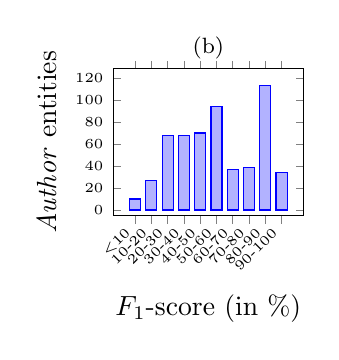
\begin{tikzpicture}[baseline=0]
        \begin{axis}[
        ybar,
        enlargelimits=0.15,
              %legend style={at={(0.5,-0.15)}, anchor=north,legend columns=-1},
        bar width=4,
        ylabel={\textit{Author} entities},
        xlabel={$F_1$-score (in \%)},
        title=(b),
        symbolic x coords={<10, 10-20, 20-30, 30-40, 40-50, 50-60, 60-70, 70-80, 80-90, 90-100},
        xtick=data,
        nodes near coords align={vertical},
        x tick label style={rotate=45,anchor=east},
        ]
        \addplot coordinates {(<10,10)
                              (10-20,27)
                              (20-30,68)
                              (30-40,68)
                              (40-50,70)
                              (50-60,94)
                              (60-70,37)
                              (70-80,39)
                              (80-90,113)
                              (90-100,34)};
        \end{axis}
      \end{tikzpicture}


 \\ %\hline
\end{tabular}
\caption{(a) \textsc{msag} cleaning: Recall and F1 values; (b) \textsc{msag} Experiments} 
\label{tab:msag}
\end{table*}

We extend the applicability of Markov logic to web data and provide initial results on cleaning the highly imperfect graph structured \textsc{MSAG} data set. We study the efficiency of data cleaning on web data by leveraging the connection between information completeness and data consistency. These two data issues interact with each other: missing values imputation helps to fix inconsistencies, and by correcting values missing entities can be identified. %In order to repair the attributes of an entity, they should not be missing and on the other hand, the data should be consistent for information completeness. \note{rewrite, sounds awkward}. -done.
In this experiment we partition our data and run inference for each author in isolation. We obtain a subgraph per \textit{Author}-entity with at least 10 \textit{Paper}-\textit{Author} edges. Next, we randomly select 600 \textit{Author}-entities. 

Table~\ref{tab:msag} (a) shows the accuracy achieved by our approach on the sample of \textsc{MSAG} dataset. We show the accuracy as relation between Recall ($x$-axis) and $F_1$-score ($y$-axis). We distinguish between three kinds of \textit{Author}-nodes (which are marked separately in Table~\ref{tab:msag} (a)): 
nodes with one or two missing \textit{Author}-\textit{Organisation} edges, nodes with three or four missing values for the \textit{Author} \textit{Organisation} connection, and finally nodes with more than 5 missing edges. Additionally, Table~\ref{tab:msag} (b) provides another perspective on this experiment by revealing the exact distribution of corrected \textit{Author}-entities ($x$-axis) by $F_1$-score ($y$-axis). The result shows the following: The method demonstrates overall $F_1$ score greater than $50\%$ and recall greater than $78\%$ for \textit{Author}-entities with one to two missing edges. Starting from three missing edges, we still achieve a good \anno{be precise, you cannot just write "good"} recall, though the precision (and therefore $F_1$ score) drops. This happens because our approach selects more false positives with an increasing number of missing values. This experiment tells us that our method produces satisfying results on web data with very little noise only (e.g., missing values). In future work, extending data cleaning rules with domain specific information should be studied further in order to reduce the false positives rate. Because the \textsc{MSAG} dataset has only recently been published and related work in data cleaning systems provide results for cleaning relational data only, we are not able to compare ourselves to another system directly.

\subsection{Impact of Rule Execution Order}
Next, we study different orders of executing data cleaning rules, to show that specifying the optimal order of rules manually is hardly achievable~\cite{Dallachiesa:2013:NCD:2463676.2465327}. We investigate whether it is beneficial to leverage joint inference for simultaneous rule execution instead of manual specification of the optimal order of data cleaning rule execution. We verify the result in Figure~\ref{fig:orderexec} by investigating the $F_1$-score ($y$-axis) distribution of various data quality settings executed on varying noise rates ($x$-axis). We run our Markov Logic program on the attributes \textsf{state} and \textsf{zip} of the \textsc{hosp} dataset because they both participate in CFD and MD. Furthermore, we fix the dataset size at ninety thousands tuples with a noise rate varying from $2\%$ to $10\%$. Each experiment consists of three parts: First, we run the MD rules and then the CFDs, which gives us the overall worst accuracy. This results agree with the previous experiment about the joint modeling data cleaning rules (c.f.,~Table~\ref{tab:plots} (a) and Section \ref{subsec:exp1}). The MD rules perform poorer than CFDs. The overall $F_1$ score ranges between $0.01$ and $0.02$, which can be explained by really low precision and recall values due to error propagation from MDs to CFDs. 
%\anno{what is poor? explain in reference to plots!}. 
In the second part of the experiment, we change the sequence of execution to running CFD rules before MD rules. This slightly improves the $F_1$ scores by increasing them from $0.1$ to $0.3$ for different noise values. We attribute this to the fact that CFDs initially detect more violations. However, analogous to the previous part, error propagation leads to the insufficient results. 

In the third and final part of the experiment, we perform the simultaneous execution of CFD and MD rules, meaning we modeled matching (for values deduplication) and repair (for erroneous values) processes together. Here we see a rapid increase of all accuracy values from $0.86$ for $2\%$ noise to $0.95$ on $10\%$ noise against the previously performed sequential execution of data cleaning rules. The growing trend of the $F_1$ scores has same explanation as results the experiment about holistic data cleaning (c.f.,~Table~\ref{tab:plots} (a) and Section \ref{subsec:exp1}) namely the functionality of the CPI algorithm. These results confirm our hypotheses that it is highly beneficial to execute multiple data cleaning rules simultaneously.  

The \textsc{nadeef} system~\cite{Dallachiesa:2013:NCD:2463676.2465327}, which also treats various types of rules holistically, ran an analogous experiment. Note that we report $F_1$-score improvements by almost $10\%$ over the values reported by \textsc{nadeef}. \note{rewrite sentence, tell readers factor of improvement as above}.
%\pgfplotsset{small,  compat=1.5}

\begin{figure}
\centering
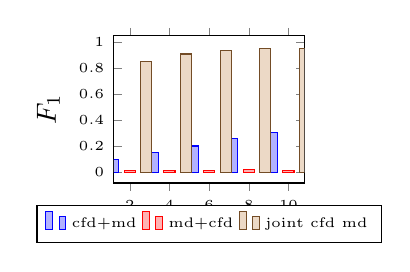
\begin{tikzpicture} 
\begin{axis}[
ybar,
enlargelimits=0.1,
legend style={at={(0.5,-0.15)}, anchor=north,legend columns=-1},
bar width=4,
ylabel={$F_1$},
symbolic x coords={2,4,6,8,10},
xtick=data,
nodes near coords align={vertical},
]
\addplot coordinates {(2, 0.1) (4, 0.1552) (6, 0.2039) (8, 0.2625) (10, 0.3048)};
\addplot coordinates {(2, 0.0176) (4, 0.0139) (6, 0.0173) (8, 0.0214) (10, 0.016)};
\addplot coordinates {(2, 0.8566) (4, 0.9114) (6, 0.9403) (8, 0.9512) (10, 0.9569)};

\legend{cfd+md,md+cfd,joint cfd md}

\end{axis}
\end{tikzpicture}
\caption{\note{Label for x axis missing!} Execution order with Markov Logic} 
\label{fig:orderexec}
\end{figure}

\subsection{Performance}

Next, we study the runtime of our method for different data sizes and noise rates. Table~\ref{tab:runtime}~(c) for \textsc{hosp} and Table~\ref{tab:runtime}~(c) (f) for \textsc{tpc-h} show the runtime values ($y$-axis) for every data size ($x$-axis) setting. Each plot denotes different noise percentages. We see that the runtime on both, real-life and synthetic data, reveals an upward trend. Cleaning datasets with joint inference will take longer the larger the data is and the more noise it contains. \note{one plot shows linear increase, the other superlinear, mention and explain this!}. This is again a characteristic of the underlying MAP inference algorithm \textit{Cutting Plane Inference} \cite{riedel08improving}: Having less noise causes the algorithm converge faster, hence faster runtime values for data with less noise. This experiment tells us that, while our method is robust against noise, but adding more noise leads to higher runtime. \anno{That is not a good finding, elaborate on the rate of runtime increase}


\subsection{Usability in Modeling Data Cleaning Rules}

%Big table containing all the rules and formulas:
\begin{table*}[t]\footnotesize
\scriptsize
\centering

\begin{tabular}{cll}
\textbf{\textit{Data Set}}               & \multicolumn{1}{c}{\textbf{\textit{Data Cleaning Rules}}}              & \multicolumn{1}{c}{\textbf{\textit{Markov Logic Formulae}}} \\ \hline
%hosp
\multirow{2}{*}{\textsc{hosp}}  & %hosp dq rules
                        \begin{tabular}[c]{@{}l@{}}
                        $\mathsf{cfd_1: \textsc{hosp}([\textsf{zip}] \rightarrow [\textsf{state, city}], t1=(\_ \parallel \_, \_))}$\\
                        $\mathsf{cfd_2: \textsc{hosp}([\textsf{phone}] \rightarrow [\textsf{addr, zip,state, city}],t2=(\_ \parallel \_,\_,\_,\_))}$
                        \end{tabular}                   
                        & %hosp markov logic cfd
                        \begin{tabular}[c]{@{}l@{}}
                        $\mathsf{w_1: \textsf{zip}(id1, code)~\wedge~\textsf{zip}(id2, code)~\wedge \textsf{state}(id1, s1)~\wedge~\textsf{state}(id2, s2)~}$ \\
                        $\mathsf{~~~~~~~~\wedge!\textsf{state}(id1, s2)~\wedge~!\textsf{state}(id2, s1)~\Rightarrow \textsf{equal-state}(id1, s1, id2, s2)}$\\
                        %second cfd:
                        $\mathsf{w_2: \textsf{zip}(id1, code)~\wedge~\textsf{zip}(id2, code)~\wedge \textsf{city}(id1, c1)~\wedge~\textsf{city}(id2, c2)~}$ \\
                        $\mathsf{~~~~~~~~\wedge!\textsf{city}(id1, c2)~\wedge~!\textsf{city}(id2, c1)~\Rightarrow \textsf{equal-city}(id1, c1, id2, c2)}$
                        \end{tabular}                 \\ 
                       & %hosp md rule
                         \begin{tabular}[c]{@{}l@{}}
                        $\mathsf{md_1: \textsc{hosp}[\textsf{zip}]=\textsc{zipcode}[\textsf{zip}]\wedge \textsc{hosp}[\textsf{state}]\neq \textsc{zipcode}[\textsf{state}]}$\\
                        $\mathsf{~~~~~~~~~~~~~~\rightarrow\textsc{hosp}[\textsf{state}]\rightleftharpoons \textsc{zipcode}[\textsf{state}]} $
                        \end{tabular}                 
                       & %hosp markov logic md
                       \begin{tabular}[c]{@{}l@{}}
                        $ todo $
                       \end{tabular}                  
                       \\ \hline

%tpc-h
\multirow{2}{*}{\textsc{tpc-h}} & %tpc-h fds
                        \begin{tabular}[c]{@{}l@{}}
                        $\mathsf{cfd_1: \textsc{t}([\textsf{c\_custkey}] \rightarrow [\textsf{c\_name,c\_address}],t1=(\_ \parallel \_, \_))} $
                        \end{tabular}                   
                        &%tpc-h mlogic fds
                         \begin{tabular}[c]{@{}l@{}}
                        $ todo $
                        \end{tabular}                    
                         \\  
                       & %tpch md rules
                       \begin{tabular}[c]{@{}l@{}}
                        $\mathsf{md_1: \textsc{t}[\textsf{c\_address}]=\textsc{t}[\textsf{c\_address}] \rightarrow \textsc{t}[\textsf{c\_phone}]\rightleftharpoons \textsc{t}[\textsf{c\_phone}]}$\\ 
                        $\mathsf{md_2: \textsc{t}[\textsf{c\_name}]=\textsc{t}[\textsf{c\_name}] \rightarrow \textsc{t}[\textsf{c\_address}]\rightleftharpoons \textsc{t}[\textsf{c\_address}]} $

                        \end{tabular}                  
                       & %tpch md markov logic
                       \begin{tabular}[c]{@{}l@{}}
                        $ todo $
                        \end{tabular}                     
                       \\ \hline
%msag
\multirow{3}{*}{\textsc{msag}}  & % msag fd
                                \begin{tabular}[c]{@{}l@{}}
                                $\mathsf{cfd_1: \textsc{m}([\textsf{author\_id, year}] \rightarrow [\textsf{affiliation\_id}],t1=(\_,\_ \parallel \_))} $\\
                                $\mathsf{cfd_2: \textsc{m}([\textsf{affiliation\_id}] \rightarrow [\textsf{origin\_name}],t2=(\_ \parallel \_))} $
                                \end{tabular}                   
                                & %msag markov logic fd
                                \begin{tabular}[c]{@{}l@{}}
                                $todo $
                                \end{tabular}                   
                                \\  
                                & % msag extended fd
                                \begin{tabular}[c]{@{}l@{}}
                                 $\mathsf{eCfd_1: \textsc{m}([\textsf{author\_id, year}] \rightarrow [\textsf{affiliation\_id}],t1=(\_, diff(\_)\leq 2 \parallel \_))} $   
                                \end{tabular}             
                                & % msag markov logic 
                                \begin{tabular}[c]{@{}l@{}}
                                $ todo $
                                \end{tabular}  
                                \\
                                &%additional predicates for msag
                                %nothing here
                                & Equality axioms:
                                \begin{tabular}[c]{@{}l@{}}
                                $symmetry$\\
                                $transitivity$
                                \end{tabular}  

                                \\ \hline
\end{tabular}
\caption{Usability in modeling data cleaning rules as Markov Logic programs.}
\label{tab:rulesformulas}
\end{table*}

\note{This section would greatly benefit from a few concrete examples that show the benefits of modeling rules with markov logic!!! Furthermore, you need to explain how you measure usability!!!}

Lastly, we focus on the feasibility of translating data quality rules into Markov logic. We conduct experiments on all three datasets described above. 

\textbf{\textsc{hosp} Quality Rules}. In our data cleaning method for the \textsc{hosp} data, we use 6 manually designed CDFs and one MD, which result in 15 normalized CFDs. One MD rule is transformed into 2 formulas. All data cleaning rules are positive. Finally, all interleaved rules are translated into 21 Markov logic formulas. In the Table \ref{tab:rulesformulas}, we provide an example of these data quality rules, which are defined on pairs of tuples. The MD rule is specified on a two relations. Markov logic predicates used for data quality formulae are shown in Table~\ref{tab:predicates}. After transforming the 100k \textsc{hosp} tuples into Markov logic grounded atoms, the resulting data comprises 1.3M evidence atoms, which will be used for inference. We empirically observe that extending the data quality rules set for for some additional conditions \anno{be specific} reduces the search space and therefore converges much faster than \textit{"pure"} model. This means that each first order logic formula, which represent the RHS of the normalized data quality rule $\mathsf{\textsf{attr}(id1, v1)~\wedge~\textsf{attr}(id2, v2)}$ becomes an inverse part $\mathsf{!\textsf{attr}(id1, v2)~\wedge~!\textsf{attr}(id2, v1)}$. This additional part denotes that we consider only tuples with different values. Here the normalized CFD rules are being compiled as demonstrated in the Table \ref{tab:rulesformulas}. \note{What has this whole paragraph to do with usability? How did you measure it? What is the purpose of this discussion?}

\textbf{\textsc{tpc-h} Quality Rules}. We write 9 CFDs and 3 MDs for this dataset. One example of the rules is a CFD that states if two tuples agree on \textsf{c\_custkey}, then they should agree on \textsf{c\_name} and \textsf{c\_address} attributes. MDs are designed on the same schema \textsc{tpc-h} \textsf{(T, T)}. These MDs state that for any pair of tuples $(t_1,t_2)$ if the LHS is similar, then the attribute values on the RHS should be identified. In the Table \ref{tab:rulesformulas} we provide an except of the data quality rules we create for \textsc{tpc-h}. Markov logic predicates used for data quality rules are shown in Table~\ref{tab:predicates}. After transforming the 100k \textsc{tpc-h} tuples into Markov logic grounded atoms, the resulting data comprises 1 Mio evidence atoms, which are then used for inference. \note{Again: What has this whole paragraph to do with usability? How did you measure it? What is the purpose of this discussion?}

\textbf{\textsc{msag} Quality Rules}. Due to the graph nature of the \textsc{msag} data (c.f.,~Figure \ref{fig:msagmissing}) we develop data quality rules, which are based on CFDs, \textit{extended} CFDs \cite{Chen2009extended} and equality axioms, such as \textit{symmetry} and \textit{transitivity}. For the \textit{Paper}-\textit{Author}-\textit{Organisation} subgraph we define two CFDs, one extended CFD and 8 additional rules that comprises equality axioms for hidden predicates. Considering the semantical meaning of the data, we profit from the ability to add supporting knowledge into data cleaning process. For example, having the CFD $\mathsf{\textsc{m}([\textsf{author\_id, year}] \rightarrow [\textsf{affiliation\_id}],t1=(\_,\_ \parallel \_))} $  allows us to capture all missing affiliation by the same author, which published in the same year. In real life we know that in academia an average contract lasts around 2-3 years. Therefore by incorporating this knowledge in form of a predicate $\mathsf{\textsf{inRange}(year, year)}$, we will extend our search range. Additionally, by combining with equality axioms, we enable capturing more missing values. For example, the hard rule $\mathsf{\textsf{equal-Affiliation}(id_1, id_2) ~\wedge~ \textsf{equal-Affiliation}(id_2, id_3) \Rightarrow  \textsf{equal-Affiliation}(id_1, id_3)}$ denotes transitive relationship between three different entities \textit{Organisation}. In total, Markov Logic program consists then from 21 lines of code. \note{Again: What has this whole paragraph to do with usability? How did you measure it? What is the purpose of this discussion?}

This part of our experimental study demonstrates that the expressiveness of Markov Logic affords us to model data cleaning rules in a convenient \anno{be more specific} manner. While existing data cleaning systems \cite{Dallachiesa:2013:NCD:2463676.2465327} are also concerned about the generality of the data cleaning rules, we can define Markov Logic data cleaning rules in expressive first-order logic manner without the need to implement any code.  Furthermore, Markov Logic is data format independent, which facilitates data cleaning on different data formats as provided on relational and graph data formats. The direct translation of data cleaning rules into first-order logic (and therefore Markov Logic formulae) simplifies the process of writing data cleaning routines. 


\subsection{Summary}
\note{Add references to the individual chapters when you summarize! Does this summary cover all experiments?}

The results of our experimental study indicate that multiple types of data cleaning rules should be considered \textit{holistically}, which confirms previous research \cite{Dallachiesa:2013:NCD:2463676.2465327, Fan:2014:IRM:2628135.2567657, Fan:2011:IRM:1989323.1989373}. Adding domain or structural knowledge about data into the Markov logic program improves overall data cleaning. Furthermore, by using joint inference we are able to achieve very good results without defining the order of the data cleaning rules execution. We find that joint modeling of data quality rules results in better \anno{be specific! you mean higher accuracy, right?} data correction. By combining matching and repairing processes, we achieve better \anno{be specific!} results than by performing these processes separately. By using the probabilistic-logical framework Markov logic we benefit from its flexibility in constraints definition and joint inference over different data repair and match rules. Therefore it is a great fit into the data quality management field; \anno{be specific, don't just claim something. Why exactly is it a great fit?}



%%%%%%%%%%%%%%%%%%%%%%%%%%%%%%%%%%%%%%%%%%%%%%%%%%%%%%%%%%%%%%%%%%%%%%%%
% Related Work
%%%%%%%%%%%%%%%%%%%%%%%%%%%%%%%%%%%%%%%%%%%%%%%%%%%%%%%%%%%%%%%%%%%%%%%%
\section{Related Work}
\label{sec:related}

Our research builds on previous work from two areas: 
\begin{inparaenum}[\itshape 1\upshape)]
\item Data quality management and
\item Statistical relational learning, namely probabilistic-logical languages.
\end{inparaenum}

\textbf{Data Quality Management}: A rich theoretical and practical investigation into data cleaning was presented in~\cite{Fan:2014:IRM:2628135.2567657} and \cite{fellegi1976systematic}. Fan W. et al.~\cite{Fan:2011:IRM:1989323.1989373} first proposed to unify the record matching and data repairing processes. They also proved that this unification greatly contributes to the improvement of the data quality. Based on this fundamental research, we propose to use probabilistic-logical frameworks to model the interaction of data quality rules and show that Markov logic enables us to simultaneously use MDs and CFDs. Holistic data cleaning methods based on integrity constraints and denial constraints with ad-hoc predicates have also been studied in \cite{chu2013holistic}. This approach considers the generalization of integrity constraints by translating them into denial constraints. However, denial constraints cannot express inclusion dependencies, hence in our work, we use the clausal form of the first-order predicate logic to express all kinds of integrity constraints. A generalization of dependencies was proposed by the Llunatic system in \cite{llunaticVDLB2013b}. They introduce a new language based on equality generated dependencies to standardize the way in which to express intra- and inter-dependencies. A clustering-based declarative approach for deduplication based on data constraints has been suggested in the Dedupalog language in \cite{Arasu:2009:LDC:1546683.1547340}.

The \textsc{Nadeeff} system from \cite{Dallachiesa:2013:NCD:2463676.2465327} is the system closest to ours with regard to the coverage of requirements for data cleaning systems. Analogous to our system, they treat data quality rules holistically. In contrast to \textsc{Nadeeff}, 
\begin{inparaenum}[\itshape 1\upshape)]
	\item we use first-order logic to define all the kinds of data quality rules and, therefore do not need black-boxes in the form of user-defined functions. Furthermore, we claim a higher usability of the system through ability to declaratively formulate rules;
	\item we perform data cleaning as an inference process on Markov networks. The inference is fully hidden from the user, which achieves a substantial complexity reduction.
\end{inparaenum}  

Relevant work in statistical inference and data cleaning has been conducted by Mayfield and his team in~\cite{Mayfield:2010:EDA:1807167.1807178}. Their system \textsc{Eracer} has been designed to perform missing values imputation. In our work, we also use statistical inference to predict missing values, repair data, and detect duplicate entries. We apply MAP inference to infer the types of errors and their sources. We also assume that the data quality rules based on FDs, CFDs, and MDs are already defined. Song and Chen, as well as Fan W. et al. present profiling algorithms to discover CFDs and MDs automatically~\cite{song2009discovering,Fan:2011:DCF:1978258.1978514}. Applying machine learning for entity deduplication has been demonstrated in \cite{guo2010record}. The work in \cite{beskales2010probclean} uses a probabilistic model for duplicate detection with uncertain outcomes. Throughout our work we use SRL, which is an extension of machine learning with respect to existing relations in the data. There are more approaches to combine logical and statistical data cleaning suggested by Prokoshyna N. et al in \cite{prokoshyna2015combining}, they apply relaxed functional dependencies (metric FDs \cite{Koudas2009MFD, caruccio2016relaxed}) as integrity constraint interface and propose a strategy to choose a high-quality minimal repair. Assessing the effectiveness of data cleaning by introducing the statistical distortion metric is investigated in \cite{dasu2012statistical}. 

The most recent work in data curation that subsumes data cleaning is the Data Timer System~\cite{Stonebraker_datacuration}. The researchers present an end-to-end system that performs massive data curation and data deduplication by combining two elements: machine learning and expert (human) feedback. In our work, we emphasize the joint execution of data cleaning rules, which are declared as \textit{soft} or \textit{hard}. Furthermore, we do not require human input to achieve high accuracy results, instead, we fully rely on the MAP-inference results to predict errors. Using machine learning and likelihood methods for cleaning noisy databases by predicting possible data updates has been introduced in \textsc{SCARE} system \cite{Yakout:2013:DSU:2463676.2463706}. In contrast to \textsc{SCARE}, our solution is capable of modeling and predicting not only missing values imputation and data consistency but also data deduplication.

Recently proposed declarative approach in \cite{burdick2015MLN} to data deduplication adopts \textit{link-to-source} constraints and theoretically proofs a connection of entity linking to a probabilistic framework based on MLN. In our work, we empirically show that MLN based data cleaning is a natural fit for solving data quality issues. 

\textbf{Statistical Relational Learning}: An advantage of probabilistic modeling for data quality has been investigated in~\cite{doi:10.1080/01621459.1972.10481323} and~\cite{chen2011usher}. Markov logic as a formalism for joint inference has been successfully used in a number of tasks, including natural language processing \cite{che2010jointly, riedel08collective, meza09jointly}, ontology alignment, data integration~\cite{niepert2011probabilistic} and co-reference resolution~\cite{poon2008joint,singla2006entity}. These research results demonstrate the advantage of joint modeling vs. pipeline execution. We are the first to apply this formalism to data cleaning and to show the benefits of a joint data cleaning approach that uses MLNs as a framework for interacting data quality rules. 



%%%%%%%%%%%%%%%%%%%%%%%%%%%%%%%%%%%%%%%%%%%%%%%%%%%%%%%%%%%%%%%%%%%%%%%%
% Conclusion
%%%%%%%%%%%%%%%%%%%%%%%%%%%%%%%%%%%%%%%%%%%%%%%%%%%%%%%%%%%%%%%%%%%%%%%%
\section{Conclusion and Future Work}
\label{sec:conclusion}
We presented a declarative data cleaning approach based on statistical relational learning and probabilistic inference. We demonstrated how functional dependencies, expressed as first-order logic formulas, are translated into probabilistic logical languages, allowing us to reason over inconsistencies or duplicates in a probabilistic way. Our approach allows the usage of probabilistic joint inference over interleaved data cleaning rules to improve data quality. By using a declarative probabilistic-logical formalism such as Markov logic, we are able to incorporate more semantic constraints and, therefore, extend traditional data quality rules. The results that we have presented in this paper indicate that taking a holistic view on data cleaning and that modeling this intuition within a Markov logic framework is a feasible and effective means to create data cleaning systems. In our future research we will focus on improving data quality for distributed and heterogeneous data sets.


\bibliographystyle{abbrv}
\bibliography{sigproc} 
\balancecolumns

\end{document}
